\subsection{Cinemàtica inversa}

El càlcul invers és el que ens serveix per trobar els angles a partir de la posició a la que volem situar la plataforma. Es pot fer el càlcul per cada motor de manera separada. Primer s'han de definir les mides principals del robot que s'utilitzaran en el càlcul.

\subsubsection{Definicions de variables}
\begin{figure}[h!]
\centering
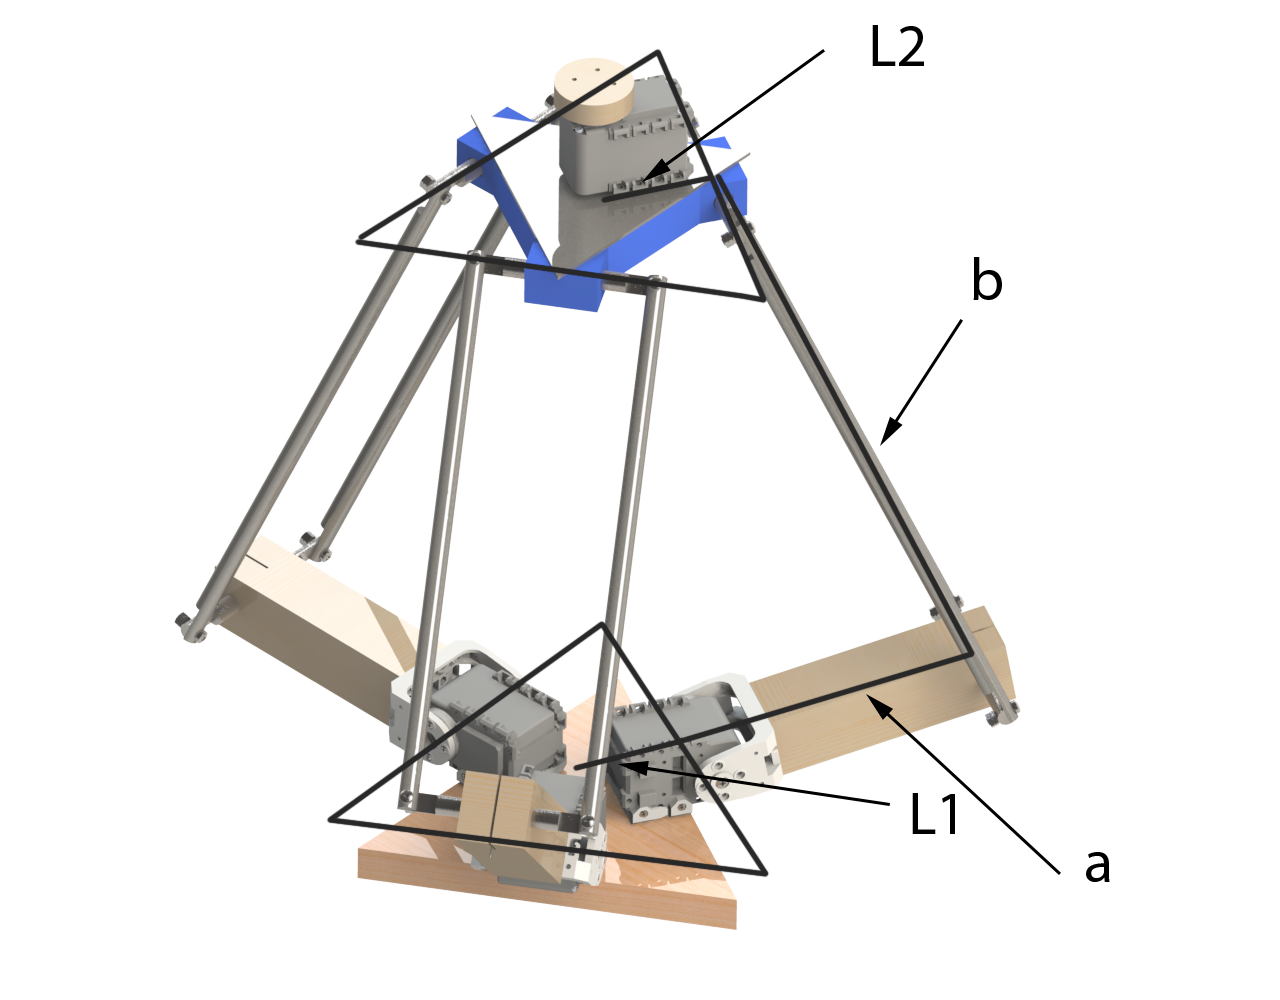
\includegraphics[width=12cm]{./imgComp/esquema_general}
\end{figure}

\begin{description}
\item[a] és la mida total del braç, des de l'eix del motor fins a l'eix de la connexió amb l'avantbraç.
\item[b] és la mida de tot l'avantbraç des de la connexió amb el braç fins a la unió amb la plataforma.
\item[L1] és la distància entre el centre de la base als eixos dels motors.
\item[L2] és la distància entre el centre de la plataforma a l'eix de connexió amb l'avantbraç.
\end{description}

\subsubsection{Càlcul d'un angle}
Si considerem que l'origen de coordenades està posicionat al centre de l'eix del motor. 


\subsubsection{Canvi de base}

\subsection{Rang de treball}

\subsection{Implementació en C++}